\PassOptionsToPackage{unicode=true}{hyperref} % options for packages loaded elsewhere
\PassOptionsToPackage{hyphens}{url}
\PassOptionsToPackage{dvipsnames,svgnames*,x11names*}{xcolor}
%
\documentclass[]{article}
\usepackage{lmodern}
\usepackage{amssymb,amsmath}
\usepackage{ifxetex,ifluatex}
\usepackage{fixltx2e} % provides \textsubscript
\ifnum 0\ifxetex 1\fi\ifluatex 1\fi=0 % if pdftex
  \usepackage[T1]{fontenc}
  \usepackage[utf8]{inputenc}
  \usepackage{textcomp} % provides euro and other symbols
\else % if luatex or xelatex
  \usepackage{unicode-math}
  \defaultfontfeatures{Ligatures=TeX,Scale=MatchLowercase}
\fi
% use upquote if available, for straight quotes in verbatim environments
\IfFileExists{upquote.sty}{\usepackage{upquote}}{}
% use microtype if available
\IfFileExists{microtype.sty}{%
\usepackage[]{microtype}
\UseMicrotypeSet[protrusion]{basicmath} % disable protrusion for tt fonts
}{}
\IfFileExists{parskip.sty}{%
\usepackage{parskip}
}{% else
\setlength{\parindent}{0pt}
\setlength{\parskip}{6pt plus 2pt minus 1pt}
}
\usepackage{xcolor}
\usepackage{hyperref}
\hypersetup{
            pdftitle={Amplify a Bayesian: Probably a Better Method for Forecasting Unanswerable Questions},
            pdfauthor={Nuño Sempere},
            colorlinks=true,
            linkcolor=Maroon,
            filecolor=Maroon,
            citecolor=Blue,
            urlcolor=blue,
            breaklinks=true}
\urlstyle{same}  % don't use monospace font for urls
\usepackage{graphicx,grffile}
\makeatletter
\def\maxwidth{\ifdim\Gin@nat@width>\linewidth\linewidth\else\Gin@nat@width\fi}
\def\maxheight{\ifdim\Gin@nat@height>\textheight\textheight\else\Gin@nat@height\fi}
\makeatother
% Scale images if necessary, so that they will not overflow the page
% margins by default, and it is still possible to overwrite the defaults
% using explicit options in \includegraphics[width, height, ...]{}
\setkeys{Gin}{width=\maxwidth,height=\maxheight,keepaspectratio}
\setlength{\emergencystretch}{3em}  % prevent overfull lines
\providecommand{\tightlist}{%
  \setlength{\itemsep}{0pt}\setlength{\parskip}{0pt}}
\setcounter{secnumdepth}{0}
% Redefines (sub)paragraphs to behave more like sections
\ifx\paragraph\undefined\else
\let\oldparagraph\paragraph
\renewcommand{\paragraph}[1]{\oldparagraph{#1}\mbox{}}
\fi
\ifx\subparagraph\undefined\else
\let\oldsubparagraph\subparagraph
\renewcommand{\subparagraph}[1]{\oldsubparagraph{#1}\mbox{}}
\fi

% set default figure placement to htbp
\makeatletter
\def\fps@figure{htbp}
\makeatother


\title{Amplify a Bayesian: Probably a Better Method for Forecasting
Unanswerable Questions}
\author{Nuño Sempere\footnote{Quantified Uncertainty Research Institute}}
\date{\today}

\begin{document}
\maketitle

\hypertarget{motivation}{%
\section{Motivation}\label{motivation}}

In \href{https://arxiv.org/abs/2106.11248}{Alignment Problems With
Current Forecasting Platforms}, Sempere and Lawsen outline a variety of
problems with current forecasting platforms, whose scoring rules are
found to either not be proper---as in the case of Good Judgment Open or
CSET-Foretell (now INFER)---or incentivize distorting one's true
probabilities to maximize the chances of placing in the top few
positions which earn a monetary reward---as in the case of Metaculus. In
addition, in almost all cases, forecasting platforms---or, for that
matter, prediction markets---disincentivize collaboration.

Against that backdrop,
\href{https://papers.ssrn.com/sol3/papers.cfm?abstract_id=3954498}{Reciprocal
Scoring: A Method for Forecasting Unanswerable Questions}, Karger et
al.~describe a method to elicit predictions in situations in which
resolutions are outright not possible, or very far away. They provide
some preliminary evidence of its effectiveness in the form of a small
randomized trial. However, in the post-peer-review discussion phase in
social media, Karger et al.'s method was met with a lukewarm reception
from the community of forecasting practitioners, which has grown to view
methods which resemble Keynesian Beauty Constests with suspicion.

In this working paper, we outline an alternative method, ``amplify a
Bayesian'', which briefly looks as follows:

\begin{itemize}
\tightlist
\item
  There is a trusted authority capable of approximate Bayesian updates
  which cares about its long-term reputation, but which has limited
  capacity
\item
  A larger contingent of forecasters submit bids to that central
  authority, and is rewarded when their bids cause the central authority
  to update.
\end{itemize}

One example of a central authority able to produce Bayesian updates
might be \href{https://www.rootclaim.com/}{Rootclaim}. Rootclaim
produces a small number of highly detailed Bayesian analysis of current
affairs, and has a strong interest in mantaining its reputation in the
long-term---on the one hand because its business model is precisely
based on mantaining an accurate long-term public track record, and on
the other hand to prove the superiority of Bayesian methods, as every
Bayesian deeply desires in her heart to do. However, Rootclaim's track
record isn't yet clear.

\hypertarget{description-of-the-method}{%
\section{Description of the method}\label{description-of-the-method}}

In the interest of brevity, we shall outline our method by means of an
example, and the example shall be the question ``Will the People's
Republic of China have annexed at least half of Taiwan by 2050?'', as
operationalized by
\href{https://www.metaculus.com/questions/5320/chinese-annexation-of-most-of-taiwan-by-2050/}{Metaculus}.

\hypertarget{a-trusted-authority-determines-a-rough-prior-to-reduce-potential-forecasting-reward}{%
\subsection{A trusted authority determines a rough prior to reduce
potential forecasting
reward}\label{a-trusted-authority-determines-a-rough-prior-to-reduce-potential-forecasting-reward}}

Taiwan has been independent of mainland China since the 25th of October
1945, i.e., 76 years into the past. Per Laplace's law, the chances that
this will change by 2050 is
\(1-(1-\frac{1}{(2021-1945)+2})^{2050-2021} \approx 31\%\). Lets take
this \(31\%\) as our Bayesian's initial probability. Note that per the
\href{https://en.wikipedia.org/wiki/Reference_class_problem}{reference
class problem}, other reference classes might have been chosen, so the
point of this prior is not to be definitive, but rather to provide a
starting point less arbitrary than 50\% from which forecaster reward
might be computed in the next steps. In the case of a patron aiming to
learn from sponsoring a forecasting tournament, the prior might
represent the patron's initial probability.

\hypertarget{forecasters-attempt-to-move-the-trusted-authoritys-prior}{%
\subsection{Forecasters attempt to move the trusted authority's
prior}\label{forecasters-attempt-to-move-the-trusted-authoritys-prior}}

Note that forecasters may also work in teams to submit arguments.

\textbf{By arguing that the prior is wrong}

Forecasters might output an argument like the following:

\begin{quote}
The \(32\%\) prior is computed with respect to Taiwan, but we have more
information than that by looking at how China has asserted control over
other outer territoritories or autonomous regions. Among these one might
count Hong Kong, Macau and Tibet (and perhaps the Xinjiang Uygur
Autonomous Region). Although the process of asserting control is more
continuous in time, if we assume for simplification purposes that it
happens in any one year, this moves our Laplace prior that another
external territory will be brought under control at
\(1-(1-\frac{4}{(2021-1945)+1})^{2050-2021} \approx 78\%\). Because
Taiwan is the only such territory left, this should be our probability
for the question.
\end{quote}

\textbf{By providing evidence about current affairs}

Forecasters might output an observation like the following:

\begin{quote}
China's current bellicosity is different from the historical norm. For
instance, China has been
\href{https://www.bbc.co.uk/news/world-asia-58794094}{sending record
number of planes over Taiwan's air defence zone}. This should increase
the probability of a successful resolution.
\end{quote}

\hypertarget{the-trusted-authority-updates-and-forecasters-are-rewarded}{%
\subsection{The trusted authority updates, and forecasters are
rewarded}\label{the-trusted-authority-updates-and-forecasters-are-rewarded}}

After receiving the updates such as above, the trusted authority makes
an approximately Bayesian update. For instance, maybe she averages the
two possible base rates, and moves from \(32\%\) to
\((32\% + 78\%)/2 = 55\%\). Then, it moves \(5\%\) from \(55\%\) to
\(60\%\) on account of the increased frequency of flights over Taiwanese
airspace.

Now, one way forecasters could be rewarded would be in proportion to the
percentage points of the update. However, this has the problem of
rewarding an update from \(1\%\) to \(2\%\) the same as an update from
\(50\%\) to \(51\%\), which seems undesirable.

One parsimonious way to solve this is by denominating updates in terms
of bits---which are the natural unit for strength of conviction, though
we will not justify this here because acquiring intuitions for why this
is the case can prove to be difficult.

For intuition, an update from \(2^{n}:1\) odds to \(2^{m}:1\) odds is an
update of \((m-n)\) bits, whose size is of \(|m-n|\) bits, where
\(|\cdot|\) represents out the absolute value. So for example, an update
from \(2^1:1\) odds \(\left(\frac{2^1}{2^1 + 1} = 66\%\right)\) to
\(2^3:1\) \(\left(\frac{2^3}{2^3 + 1} = 88\%\right)\) odds corresponds
to an update from 1 bit to 3 bits, i.e., an update size of 2 bits.
Conversely, an update from \(1:2\)
\(\left(1:2 \text{ is equivalent to } 2^{-1}:1, \text{ so } \frac{2^{-1}}{2^{-1} + 1} = 33\%\right)\)
to \(2^{2}:1\) \(\left(\frac{2^2}{2^2 + 1} = 80\%\right)\) corresponds
to an update from -1 bit to 2 bits, i.e.~an update of 3 bits.

Continuing to our example, the original probability of \(32\%\)
corresponds to around \(1:2^1\) odds, or \(2^{-1}:1\) odds, or strength
of conviction of around -1 bit. The posterior probability of \(55\%\)
corresponds to around \(1.22 : 1\) odds, or around \(2^{0.3} : 1\) odds,
or +0.3 bits. The difference between these is (0.3-(-1)) = 1.3 bits. An
update from \(55\%\) to \(60\%\) would likewise be an update from
\(2^{0.3}:1\) to \(2^{0.6}:1\), or 0.3 bits.

If we valued each bit of information about an invasion of Taiwan at
\$1000, the first forecaster would receive \$1,290, while the second
would receive \$300.

Note that under this method, if the trusted authority then moved back to
\(55\%\) because of a third argument brought in by a third person, that
third person would receive \$300, but rewards already given out would
not be taken back.

\hypertarget{discussion-of-the-method}{%
\section{Discussion of the method}\label{discussion-of-the-method}}

\hypertarget{more-on-the-central-authority}{%
\subsection{More on the central
authority}\label{more-on-the-central-authority}}

When implementing this method, one might actually hire the real-life
Rootclaim. Alternatively, one might consider more than one central
authority, and aggregate forecaster rewards using some weighted average.
In practice, one or a group of excellent forecasters might also serve as
such a central authority capable of forecasting. A central authority
must be trusted, truth-seeking and unbiased for this method to work
well; in practice it may be difficult to find authoriities that are
trusted by all or most forecasters.

Throughout, we have also been using the phrase ``approximately
Bayesian''. But some updates, such as realizing that one's \emph{prior}
is wrong or incorrect, are only clumsily modelled as Bayesian.
Alternatively, updates from ``thinking more about it'', or ``making a
calibration adjustment'' do not neatly fit into the Bayesian paradigm
either. Further, updates for surprising events which not predicted with
any probability by (e.g., imagine making a Bayesian update on the advent
of nuclear weapons as a Japanese who wasn't keeping up with the physics
of the 20th century) cannot, strictly speaking, be Bayesian.
Nevertheless, we might still update a more generalized set of updates,
which includes the aforementioned but not other, arbitrary updates. On
this topic, see
\href{https://www.lesswrong.com/posts/xJyY5QkQvNJpZLJRo/radical-probabilism-1}{Radical
Probabilism} and
\href{https://www.lesswrong.com/posts/vpvLqinp4FoigqvKy/reflective-bayesianism}{Reflective
Bayesianism}.

Implicitly, we have been presenting this central authority as more
trustworthy, or more truth-seeking than the other forecasters which are
used to amplify it. But this might not necessarily be the case at all:
this method might be used as a cost-saving device instead. For instance,
maybe some forecasters are more willing to receive rewards later rather
than immediately, but both sets of forecasters produce similar quality
forecasts. Alternatively, perhaps all forecasters have similar discount
rates, but rewarding many forecasters for predictions which will be
resolved long into the future might be too expensive. In that case,
tournament designers might arbitrarily divide a tournament's cohort into
forecasters rewarded now and authorities which are rewarded later, with
the former attempting to predict and give information to the latter.

Note that this amplification method might go very wrong if forecasting
something such as ``Will the US dollar suffer from large amounts of
inflation?''. In that case, forecasters' who have reason to believe in
inflation might self-select into the group which gets rewarded now (in
dollars), and likewise forecasters with beliefs about lack of inflation
might self-select into the group which gets rewards later. In that case,
the first group of short-termists might sneakily predict that the second
group will think that there will be no inflation, but the link between
the forecasting system and reality would have been weakened.

\hypertarget{incentive-issues-for-forecasters}{%
\subsection{Incentive issues for
forecasters}\label{incentive-issues-for-forecasters}}

One more problem which might arise from the system of incentives which
we have just described might be that forecasters simply spam the trusted
authority with a large number of claims and sources, and wait for the
trusted authority to filter them. This could be fixed by requiring
inputs to be well-formed and well-written, or that we might not accept
inputs which move the trusted authority by too small an amount, i.e., by
rejecting inputs which are too ``lazy''. One could also make forecasters
pay a small price for suggesting inputs, or only give forecasters a
chance to give a finite number of inputs, which would also incentivize
well-formed and well-structured inputs.

Another problem that might arise is that forecasters will be
incentivized to exaggerate the weight of the evidence they are
presenting, to get more reward from the central authority.

But there is another potential twist which might alleviate both of these
problems, in addition to leading to further efficiency gains: Have
forecasters also try to predict how much the trusted authority will be
moved by every argument they
bring\footnote{Note that this would require fixing the ordering of each new argument/piece of evidence},
and be rewarded for being accurate in that assessment in addition to
being rewarded for bringing in new evidence. This may also incentivize
forecasters to bring up any counter-evidence to exaggreated claims, and
forecasters who consistently overexaggerate their claims could be
penalized.

For instance, one forecaster might bring up the piece of evidence we
mentioned above:

\begin{quote}
\begin{quote}
China's current bellicosity is different from the historical norm. For
instance, China has been
\href{https://www.bbc.co.uk/news/world-asia-58794094}{sending record
number of planes over Taiwan's air defence zone}. This should increase
the probability of a successful resolution.
\end{quote}
\end{quote}

And another forecaster might receive a small reward for accuracy in
predicting how much the trusted authority would update after viewing
that piece of evidence.

At this point, we have a methodology for bringing in new pieces of
evidence and judging how much to update on them by, but it requires the
trusted authority to look at each of them. However, the trusted
authority---our expensive but trustworthy Bayesian approximator---could
look at only a fraction of them, say 10\%, chosen randomly, but increase
the rewards for those predictions tenfold. Depending on the setup, this
might preserve incentive compatibility but allow us to trade off the
trusted authority's more expensive procedure for the less expensive
procedure of using forecasters. For more on this method, see
\href{https://www.lesswrong.com/posts/cLtdcxu9E4noRSons/part-1-amplifying-generalist-research-via-forecasting}{Amplifying
generalist research via forecasting} (and
\href{https://www.lesswrong.com/posts/FeE9nR7RPZrLtsYzD/part-2-amplifying-generalist-research-via-forecasting}{part
2}).

One more issue is that this method may underweight the value of
contributions which increase the resilience of the Bayesian's forecast
but don't necessarily shift it a lot. For example, it may be more
valuable to increase the resilience of a 50\% forecast from a 90\%
confidence interval (e.g.~defined as what the authority would predict
after 1,000 more hours more hours of research) of 10-90\% to a more
resilient 50\% with an interval of 40-60\%, compared to shifting the
best-guess forecast to 53\% while leaving the resilience approximately
similar (let's say, 11-91\%).

\hypertarget{evidence-base-and-comparison-to-karger-et-al.s-method}{%
\subsection{Evidence base and comparison to Karger et al.'s
method}\label{evidence-base-and-comparison-to-karger-et-al.s-method}}

On the one hand, most of the reasons why I think why this method might
be superior come from first principles reasoning or from my experience
with forecasting. With regards to first-principle reasoning, reasoning
analogous to that of
\href{https://meteuphoric.com/2014/07/21/how-to-buy-a-truth-from-a-liar/}{how
to buy truth from a liar} implies that this method will eventually
converge at the truth. To elaborate, the way for researchers to extract
maximum reward from the Bayesian approximator is by feeding it as much
evidence as they can. Further, it just feels more elegant.

With regards to evidence from my experience as a forecaster, it just
feels more grounded. Forecasters try to predict or amplify a trusted
Bayesian approximator, and the trusted Bayesian approximator tries to
predict reality. If a forecaster has unique information, they can and
should try to convince the Bayesian approximator. If the evidence is
just very private or hard to communicate, the forecaster with that
information could offer a bet to the Bayesian approximator. Forecasters
are incentivized to conduct expensive searches (e.g., interviews with
citizens of far-away lands),
cf.~\href{https://twitter.com/LinchZhang/status/1455759586158268417}{Linch
Zhang}.

\begin{figure}
\centering
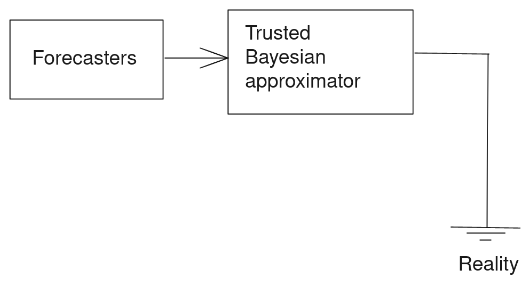
\includegraphics[width=0.5\textwidth,height=\textheight]{diagrams/amplification-diagram-1.png}
\caption{Proposed design}
\end{figure}

In contrast, Karger's method has weird loops; teams are not aiming to
forecast reality, but rather to forecast what the other team will
forecast that one's team will forecast that the other team will
forecast\ldots{} In the presence of Schelling points, human biases,
laziness, etc., it is not clear that this process converges to the
truth. For instance, the forecaster which puts in the most research
effort, or the group which puts in the most effort, is disadvantaged:
ideally, both groups want to put in the same amount of effort, or,
equivalently, find out the same things.

Some of the authors in Karger et al.'s paper bring forward the argument
that if one has larger enough teams, each person should expect and
equivalent someone in the other team to find the same evidence. Although
perhaps true in the limit, this in my experience does not seem likely to
be true in any degree of practice.

\begin{figure}
\centering
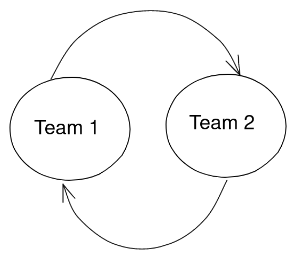
\includegraphics[width=0.3\textwidth,height=\textheight]{diagrams/amplification-diagram-2.png}
\caption{Karger et al.'s design}
\end{figure}

Although both Karger et al.'s and our method output a legible output, in
Karger's case this is a wiki, and in our case this is an approximate
Bayesian calculation. We believe that a Bayesian calculation probably is
the most legible of the two outputs. In particular, one can tweak only
some of the inputs and see how the outputs change, which would be more
difficult to do in a wiki.

\hypertarget{conclusion}{%
\section{Conclusion}\label{conclusion}}

In conclusion, the proposed method of amplifying an expensive but
Bayesian approximator has the benefit of appearing more grounded, and
not having the weird loops in Karger et al.'s reciprocal scoring
proposal---or in other Keynesian beauty contest designs. We look forward
to someone implementing the method.

\end{document}
